%%%%%%%%%%%%%%%%%%%%%%%%%%%%%%%%%%%%%%%%%%%%%%%%%%%%%%%%%%%%%%%
%
% Welcome to Overleaf --- just edit your LaTeX on the left,
% and we'll compile it for you on the right. If you open the
% 'Share' menu, you can invite other users to edit at the same
% time. See www.overleaf.com/learn for more info. Enjoy!
%
%%%%%%%%%%%%%%%%%%%%%%%%%%%%%%%%%%%%%%%%%%%%%%%%%%%%%%%%%%%%%%%


% Inbuilt themes in beamer
\documentclass{beamer}

% Theme choice:
\usetheme{CambridgeUS}

\setbeamertemplate{caption}[numbered]{}

\usepackage{enumitem}
\usepackage{tfrupee}
\usepackage{amsmath}
\usepackage{amssymb}
\usepackage{gensymb}
\usepackage{graphicx}
\usepackage{txfonts}

\def\inputGnumericTable{}

\usepackage[latin1]{inputenc}                                 
\usepackage{color}                                            
\usepackage{array}                                            
\usepackage{longtable}                                        
\usepackage{calc}                                             
\usepackage{multirow}                                         
\usepackage{hhline}                                           
\usepackage{ifthen}
\usepackage{caption} 
\captionsetup[table]{skip=3pt}  
\providecommand{\pr}[1]{\ensuremath{\Pr\left(#1\right)}}
\providecommand{\cbrak}[1]{\ensuremath{\left\{#1\right\}}}
\renewcommand{\thefigure}{\arabic{table}}
\renewcommand{\thetable}{\arabic{table}}

% Title page details: 
\title{AI1110: Assignment 9} 
\author{Aryan Sharan Reddy\\BT21BTECH11002}
\date{\today}
%\logo{\large \LaTeX{}}

\providecommand{\pr}[1]{\ensuremath{\Pr\left(#1\right)}}

\begin{document}

% Title page frame
\begin{frame}
    \titlepage 
\end{frame}

% Remove logo from the next slides
%\logo{}


% Outline frame
\begin{frame}{Outline}
    \tableofcontents
\end{frame}


% Lists frame
\section{Question}
\begin{frame}{Question}
The input to the system

\begin{center}
    H(s)=\dfrac{1}{s^2+2s+5}\\
\end{center}

is a WSS  process x(t) with $E\{x^2(t)\}=10$. Find $S_{x}(\omega)$ such that the average power $E\{y^{2}(t)\}$ of the resulting output $y(t)$ is maximum.
\\
(\textit{Hint:} $|H(j\omega)|$ is maximum for $\omega=\sqrt{3}$)
\end{frame}

\section{Solution}
\begin{frame}{Solution}
In general
\begin{align}
    E\{y^{2}(t)\} &= \dfrac{1}{2\pi} \int_{-\infty}^{\infty} S_{x}(\omega)|H(\omega)|^{2}d\omega\\
                &\leq |H(\omega_{m})|^{2} \dfrac{1}{2\pi}\int_{-\infty}^{\infty} S_{x}(\omega)d\omega\\
                &= E\{x^{2}(t)\} |H(\omega_{m})|^{2}
\end{align}
where $|H(\omega_{m})|$ is the maximum of $|H(\omega)|$. In our case ,
\begin{equation}
    |H(\omega)|^{2} = \dfrac{1}{(5-\omega)^2 + (2\omega)^2}
\end{equation}
From the hint, $|H(\omega)|$ is maximum at $\omega=\sqrt{3}$
\end{frame}

\section{Solution(Contd..)}
\begin{frame}{Solution(Contd..)}
Also $|H(\omega_{m})|^{2}=\dfrac{1}{16}$. Hence $E\{y^{2}(t)\} \leq \dfrac{10}{16}$ with the equality if R_{x}(10)=10\cos \sqrt{3}\tau 

\begin{figure}[!ht]
        \centering
        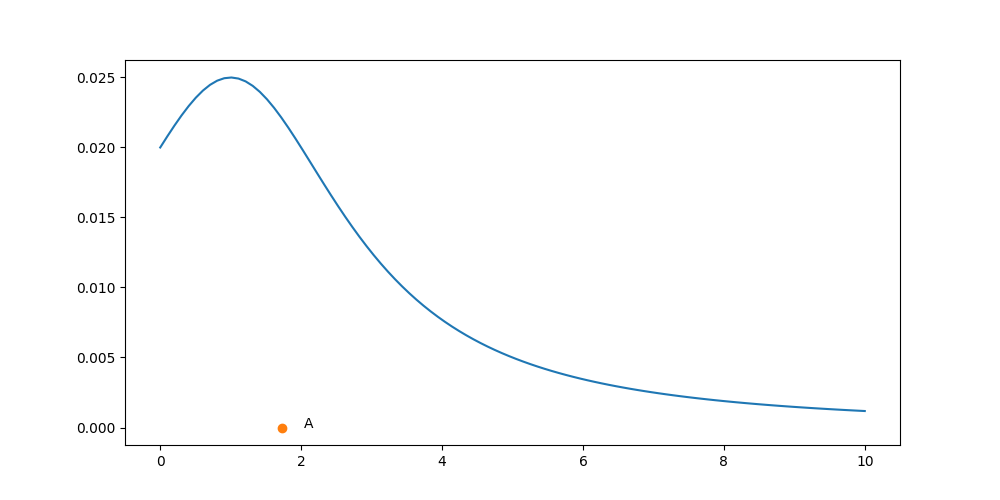
\includegraphics[width=\columnwidth]{Figure.png}
        \caption{figure shows the |H(\omega)| vs \omega plot }
        \label{fig-1}
        \end{figure}
\end{frame}
\end{document}
